\part{Model Gen~6}

\chapter{Zadanie, dane i etykiety}\label{rozdz:dane}

\section{Co dokładnie ma zrobić model?}

Mamy nagranie gitary. Chcemy dostać \emph{listę nut}: dla każdej nuty wysokość (numer MIDI), moment początku, moment końca, a jeśli się da, strunę i próg, na których ją zagrano.
Dziedzina nazywa się automatyczną transkrypcją muzyki (AMT). Dla gitary są w niej dwie szczególne trudności, które omawialiśmy w rozdziałach~\ref{rozdz:alikwoty}--\ref{rozdz:hcqt}:
wielogłosowość (kilka nut naraz i wspólne alikwoty) oraz niejednoznaczność tabulatury (ta sama wysokość na kilku strunach).

Po tym rozdziale umiesz: (i)~wskazać, ile pozycji na gryfie odpowiada danej wysokości, (ii)~policzyć mapy celów dla jednej nuty, (iii)~uzasadnić, że klatka początku zawsze „brzmi”, (iv)~wyjaśnić, po co są maski dostępności etykiet.

\section{Niejednoznaczność tabulatury}

\haslo{tabulatura}
\begin{definicja}[Pozycja na gryfie]\label{def:pozycja}
Gitara ma struny numerowane $i=1,\dots,6$ od najcieńszej ($o_1=64$, E4) do najgrubszej ($o_6=40$, E2), gdzie $o_i$ to wysokość MIDI struny pustej.
\emph{Pozycją} nuty $m$ nazywamy parę $(i,f)$ taką, że próg $f=m-o_i$ jest całkowity i $0\le f\le19$ (model zakłada progi $0$--$19$).
\end{definicja}

\begin{przyklad}\label{prz:pozycje-e4}
Nuta E4 ($m=64$) ma $64-o_i=0;\,5;\,9;\,14;\,19;\,24$ dla $i=1,\dots,6$. Próg $24>19$ odpada, więc są \emph{pięć} pozycji: struna~1 próg~0, struna~2 próg~5, struna~3 próg~9, struna~4 próg~14, struna~5 próg~19
(rys.~\ref{rys:gryf}). Nuta E2 ($m=40$) ma tylko jedną pozycję (struna~6, próg~0).
\end{przyklad}

\begin{figure}[ht]
\centering
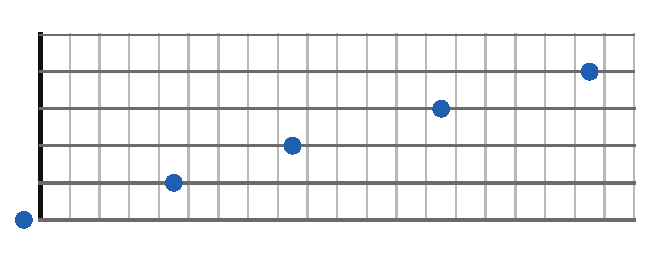
\includegraphics[width=\linewidth]{figures/gryf-e4.pdf}
\sidecaption{Gryf z $20$ progami; struny od najcieńszej (góra) do najgrubszej (dół). Niebieskie kropki to wszystkie pięć pozycji nuty E4: próg~0 (struna pusta, kropka przed siodełkiem), $5$, $9$, $14$ i $19$. Wysokość nie wystarcza do ustalenia pozycji;
o strunie decyduje barwa dźwięku (struny o różnej grubości mają inny rozkład alikwotów) i kontekst muzyczny. \label{rys:gryf}}
\end{figure}

\begin{intuicja}
Wysokość mówi „co”, tabulatura mówi „jak to zagrać”. Ta sama nuta zagrana na grubej strunie wysoko na gryfie brzmi ciemniej niż na cienkiej strunie nisko: ma inną proporcję alikwotów (rozdział~\ref{rozdz:alikwoty}).
Model może więc wnioskować strunę z widma, ale nie z samej wysokości.
\end{intuicja}

\begin{naliczbach}
Liczba pozycji nuty $m$ to $\#\{i:0\le m-o_i\le19\}$. Dla $m=40,\dots,44$ wynosi $1$; dla $m=59$ i $m=64$ jest największa i wynosi $5$; dla $m=79,\dots,83$ znów $1$.
Z $44$ wysokości $40,\dots,83$ aż $34$ ma co najmniej dwie pozycje. Tabulatura nie jest więc dodatkiem, tylko osobnym problemem: sama lista wysokości zostawia wiele wyborów (zob.\ rozdział~\ref{rozdz:dekoder}, wybór struny).
\end{naliczbach}

\section{Dane uczące}

Gen~6 uczono na danych trzech rodzajów. Wszystkie mają tę samą postać: lista nut z wysokością, początkiem i końcem (czasem struną i progiem), plus nagranie.

\begin{table}[ht]
\centering\small
\begin{tabular}{@{}p{3.1cm}p{2.3cm}p{5.2cm}@{}}
\toprule
zbiór & nagrań (ucz./walid./test) & opis\\
\midrule
klasyka, zestaw 1 & $5502/450/520$ & utwory z korpusu MIDI zagrane syntezatorem na $27$ instrumentach w $11$ miejscach, $4$ formy utworu\\
klasyka, zestaw 2 & $9135$ (tylko ucz.) & inne ziarna losowe: transpozycje, tempa, obsady\\
środowiska gitarowe & $888$ & gitara w losowym pokoju z szumem, brumem i stukami\\
GuitarSet & $168/12/180$ & prawdziwa gitara; gracze $00$--$02$ uczenie, funk gracza $02$ walidacja, gracze $03$--$05$ test\\
\bottomrule
\end{tabular}
\caption{Zbiory danych Gen~6 (ok.\ $16\,850$ nagrań, z czego do uczenia ok.\ $15\,600$). Źródło: dokumentacja projektu (\texttt{docs/WYNIKI.md}). Korpus MIDI ma $3236$ utworów ($282$ h, $8{,}2$ mln nut): MAESTRO v3 i partytury z biblioteki music21.}
\label{tab:dane}
\end{table}

\begin{pulapka}
\textbf{Tylko GuitarSet to prawdziwa gitara}, a stanowi niewielką część danych ($168$ nagrań uczących). Większość pozostałych to \emph{synteza}: nagrania generowane programem z nut. To ważne przy ocenie wyników (rozdział~\ref{rozdz:wyniki}): dobry wynik na syntezie nie dowodzi,
że model równie dobrze zadziała na każdej prawdziwej gitarze, mikrofonie i pokoju. Podział na zbiory robiono \emph{po utworach i po graczach}: utwór czy gracz z testu nigdy nie występuje w uczeniu.
\end{pulapka}

\section{Mapy celów}

Sieć zwraca dla każdej klatki $t$ i półtonu $s=m-36$ liczby $p_\mathrm{on},p_\mathrm{fr},p_\mathrm{off}\in(0,1)$ oraz inne (rozdział~\ref{rozdz:uwaga-wys}). Żeby ją uczyć, trzeba z listy nut zbudować takie same mapy \emph{wzorcowe}
$y_\mathrm{on},y_\mathrm{fr},y_\mathrm{off}$. Niech $\tau_t=(256\,t+2048)/11\,025$ będzie środkiem czasowym klatki $t$ (środek okna długiego, rozdział~\ref{rozdz:hcqt}) i $\Delta=256/11\,025=23{,}2\ms$.

\haslo{mapy celów}
\begin{definicja}[Mapy celów]\label{def:mapy-celow}
Dla nuty o wysokości $m$, początku $t_\mathrm{on}$ i końcu $t_\mathrm{end}$ niech $s=m-36$ i $k_\mathrm{on}=\round\big((t_\mathrm{on}f_s-2048)/256\big)$, $k_\mathrm{off}=\round\big((t_\mathrm{end}f_s-2048)/256\big)$, gdzie $f_s=11\,025\Hz$. Wtedy:
\begin{itemize}
\item \emph{brzmi:} $y_\mathrm{fr}(t,s)=1\iff t_\mathrm{on}-\tfrac12\Delta\le\tau_t\le\max(t_\mathrm{end},t_\mathrm{on})$;
\item \emph{początek:} $y_\mathrm{on}(k_\mathrm{on},s)=1$ i $y_\mathrm{on}(k_\mathrm{on}\pm1,s)=0{,}4$ (miękkie sąsiedztwo);
\item \emph{koniec:} tak samo, z $k_\mathrm{off}$.
\end{itemize}
Gdy nuty się nakładają, bierzemy maksimum; poza tym wartości są $0$.
\end{definicja}

\begin{przyklad}[Jedna nuta policzona do końca]\label{prz:mapy-e4}
Nuta E4 ($m=64$, $s=28$) zaczyna się w $t_\mathrm{on}=1{,}000$~s i kończy w $t_\mathrm{end}=1{,}400$~s. Wtedy
$k_\mathrm{on}=\round\big((11\,025-2048)/256\big)=\round(35{,}07)=35$, więc $y_\mathrm{on}$ w klatkach $34,35,36$ wynosi $0{,}4;\ 1;\ 0{,}4$.
Brzmi od $\tau_t\ge1{,}000-0{,}0116=0{,}9884$ s: klatka $34$ ma $\tau=0{,}9752$ (jeszcze nie), klatka $35$ ma $\tau=0{,}9985$ (tak), więc od $t=35$.
Do $\tau_t\le1{,}4$: $\tau_{52}=1{,}3932$ (tak), $\tau_{53}=1{,}4164$ (nie), więc do $t=52$. Koniec: $k_\mathrm{off}=\round(52{,}29)=52$, wartości $0{,}4;1;0{,}4$ w klatkach $51,52,53$.
Jeśli ta nuta jest grana na strunie~2 ($o=59$), próg to $64-59=5$, czyli klasa tabulatury $1+5=6$ na strunie~2 w klatkach $35$--$52$, a na pozostałych strunach $0$ (milczą).
\end{przyklad}

\begin{figure*}[ht]
\centering
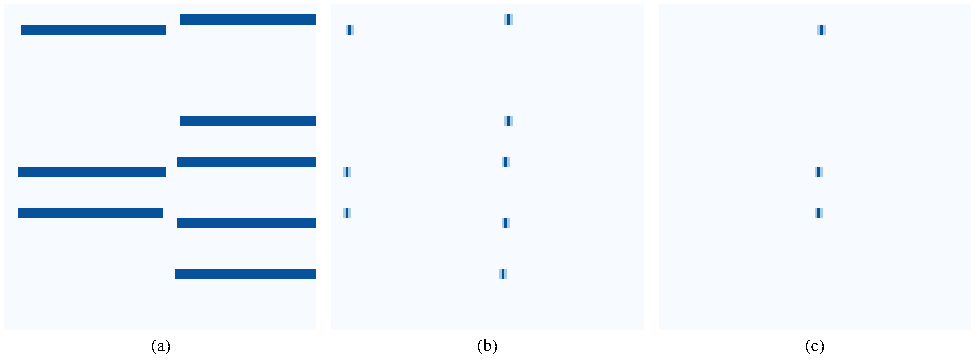
\includegraphics[width=\linewidth]{figures/mapy-celow.pdf}
\caption{Mapy celów syntetycznego nagrania z $15$ nutami (fragment: $110$ klatek, półtony $4$--$35$): (a) „brzmi” --- poziome kreski trwających nut, (b) początki --- pojedyncze kropki (jasne punkty to $1$, ich pionowe sąsiedztwo w czasie to miękkie $0{,}4$), (c) końce.
Mapy początków i końców są rzadkie: tylko $0{,}12\%$ komórek początków jest równa $1$ (rozdział~\ref{rozdz:strata}). Mapy zbudowane kodem z repozytorium.}
\label{rys:mapy-celow}
\end{figure*}

\begin{twierdzenie}[Klatka początku zawsze brzmi]\label{tw:poczatek-brzmi}
Niech nuta trwa co najmniej $\tfrac12\Delta$. Dla $k_\mathrm{on}$ z def.~\ref{def:mapy-celow} zachodzi $y_\mathrm{fr}(k_\mathrm{on},s)=1$.
\end{twierdzenie}
\begin{pomyslDowodu}
Zaokrąglenie przesuwa indeks o co najwyżej $\tfrac12$ klatki, więc środek klatki początku leży nie dalej niż $\tfrac12\Delta$ od $t_\mathrm{on}$ --- czyli mieści się w oknie definicji.
\end{pomyslDowodu}
\begin{proof}
Niech $x=(t_\mathrm{on}f_s-2048)/256$, więc $k_\mathrm{on}=\round(x)$ i $|k_\mathrm{on}-x|\le\tfrac12$. Środek klatki $k_\mathrm{on}$:
\begin{align*}
\tau_{k_\mathrm{on}}-t_\mathrm{on} &= \frac{256k_\mathrm{on}+2048}{f_s}-\frac{256x+2048}{f_s} && \pow{(def.\ $\tau$, $x$)}\\
 &= \frac{256}{f_s}\,(k_\mathrm{on}-x)=\Delta\,(k_\mathrm{on}-x). && \pow{(upraszczanie)}
\end{align*}
Zatem $|\tau_{k_\mathrm{on}}-t_\mathrm{on}|\le\tfrac12\Delta$, czyli $\tau_{k_\mathrm{on}}\ge t_\mathrm{on}-\tfrac12\Delta$ (dolna granica). Górna: $\tau_{k_\mathrm{on}}\le t_\mathrm{on}+\tfrac12\Delta\le t_\mathrm{end}$ z założenia o długości nuty. Obie nierówności zachodzą, więc $y_\mathrm{fr}=1$. To kończy dowód.
\end{proof}

W zwykłym języku: nie ma nut, które mają początek, ale „nie brzmią” w tej samej klatce. W poprzedniej generacji (Gen~5) warunek zaczynał się od $\tau_t\ge t_\mathrm{on}$, więc klatka początku mogła mieć $y_\mathrm{fr}=0$, a dekoder wymaga $p_\mathrm{fr}$ w klatce początku (rozdział~\ref{rozdz:dekoder}); taka nuta była gubiona.

\begin{intuicja}
Miękkie sąsiedztwo $0{,}4$ wokół początku mówi sieci: „nie jesteś karana za pomyłkę o jedną klatkę ($23\ms$)”. Dokładność czasowa człowieka i etykiet jest rzędu dziesiątek milisekund, a ocena przyjmuje tolerancję $50\ms$.
Z twierdzenia~\ref{tw:kalibracja} wiemy, że przy BCE etykieta $0{,}4$ uczy wyniku $\approx0{,}4$.
\end{intuicja}

\section{Dostępność etykiet}

Nie każde źródło ma wszystkie etykiety: GuitarSet ma struny i progi, ale nie głośności; korpus MIDI ma głośności i brak strun na gitarze; przy niektórych danych brak końców. Każdy przykład niesie więc wektor
$\vect a\in\{0,1\}^5$ (które z pięciu głowic: początek, brzmi, koniec, głośność, tabulatura ma \emph{naprawdę} zaadnotowane), a strata danej głowicy jest mnożona przez $a_\mathrm{głowica}$ (rozdział~\ref{rozdz:uczenie}). Dzięki temu można
łączyć źródła o różnych adnotacjach bez udawania, że brakujące etykiety są zerami.

\begin{pulapka}
Uczenie na brakujących etykietach traktowanych jako zera \emph{aktywnie szkodzi}: model uczy się, że „tu nie ma nuty”, a nie że „tu nie wiemy”. Maska dostępności jest tanim sposobem, by tego uniknąć. W Gen~6 żadne źródło nie ma etykiet głośności, więc głowica głośności pozostała nieuczona (jej wyjście nie jest zwracane).
\end{pulapka}

\section*{Podsumowanie}
\begin{itemize}
\item Wynik modelu to lista nut; wysokość nie wyznacza tabulatury ($34$ z $44$ wysokości mają $\ge2$ pozycje).
\item Dane to głównie synteza ($\approx16\,850$ nagrań) i niewielki zbiór prawdziwej gitary (GuitarSet); testujemy na utworach i graczach nieobecnych w uczeniu.
\item Mapy celów: \emph{brzmi}, \emph{początek} i \emph{koniec} (z miękkim sąsiedztwem $0{,}4$) oraz klasa tabulatury $0\ldots20$ na strunę.
\item Klatka początku zawsze też „brzmi” (tw.~\ref{tw:poczatek-brzmi}), co poprawiono względem Gen~5.
\item Maski dostępności pozwalają łączyć dane o różnych adnotacjach.
\end{itemize}

\begin{sprawdz}
\begin{enumerate}
\item Podaj wszystkie pozycje $(i,f)$ nuty $m=55$ (G3). Ile ich jest?
\item Nuta A3 ($m=57$) zaczyna się w $t_\mathrm{on}=2{,}000$~s i kończy w $t_\mathrm{end}=2{,}500$~s. Policz $k_\mathrm{on}$, $k_\mathrm{off}$ i pierwszą klatkę, w której $y_\mathrm{fr}=1$.
\item Pokaż, że mapa początków dla jednej nuty ma sumę $1+2\cdot0{,}4=1{,}8$ (dla nuty bez nakładania z innymi).
\item Dlaczego przy mapie „brzmi” w Gen~5 (start $\tau_t\ge t_\mathrm{on}$) klatka początku mogła mieć etykietę $0$? Podaj przykład liczbowy.
\end{enumerate}
\end{sprawdz}

\subsection*{Rozwiązania}
\begin{enumerate}
\item $55-o_i=-9;\,-4;\,0;\,5;\,10;\,15$ dla $i=1..6$ ($o=64,59,55,50,45,40$): dopuszczalne $0$ (struna~3), $5$ (struna~4), $10$ (struna~5), $15$ (struna~6), a ujemne odpadają. Cztery pozycje: $(3,0),(4,5),(5,10),(6,15)$.
\item $k_\mathrm{on}=\round((2\cdot11\,025-2048)/256)=\round(78{,}13)=78$; $k_\mathrm{off}=\round((2{,}5\cdot11\,025-2048)/256)=\round(99{,}67)=100$. Dolna granica $\tau_t\ge2{,}0-0{,}0116=1{,}9884$: $\tau_{78}=(78\cdot256+2048)/11\,025=1{,}9969$ (tak), $\tau_{77}=1{,}9737$ (nie). Pierwsza klatka to $78$.
\item W $k_\mathrm{on}$ wartość $1$, w $k_\mathrm{on}\pm1$ po $0{,}4$ (przy założeniu, że obie klatki mieszczą się w nagraniu i nie nakładają się inne nuty): suma $1+0{,}4+0{,}4=1{,}8$.
\item Dla $t_\mathrm{on}=1{,}000$ klatka początku $k=35$ ma środek $\tau_{35}=0{,}9985<1{,}000$, więc przy warunku $\tau_t\ge t_\mathrm{on}$ miałaby etykietę $0$; dopiero przesunięcie granicy o $\tfrac12\Delta$ ($0{,}9884\le0{,}9985$) daje $1$.
\end{enumerate}
